%------------------------------------------------------------------------%
\chapter{Metal-semiconductor junction}
%------------------------------------------------------------------------%
Metal-semiconductor junctions can be divided in 2 categories: ohmic contacts ,that are what we've called "a good contact", and rectifing devices ,that work like diodes. A good contact is a low parasitic resistance device with 2 pin through wich can flow a lot of J with a small V. Rectifing devices let current flow only in one direction, for this type of device is needed a low doped semiconductor and a metal with a proper work function; this type of devices are called Schottky diodes.

%------------------------------------------------------------------------%
\section{Schottky diode}
%------------------------------------------------------------------------%
We will study the electrostatic of this device as we've done with diodes. We initially suppose the 2 zones isolated and under thermodinamic equilibrium. Let's take the semiconductor n-doped.\\
For the metal we're not interested in the conduction or valence band but only in the position of the Fermi level. All type of material's bands are refered to the vacuum level. The distance between the Fermi-level of the metal and the vacuum level $E_0$ is calle work-function $\phi_m$. For silicon we can define the electron affinity that is the distance between the conduction band and the vacuum level $\chi_s$. In this way we can allign the two materials like in figure.\\

\begin{wrapfigure}{i}{0pt}
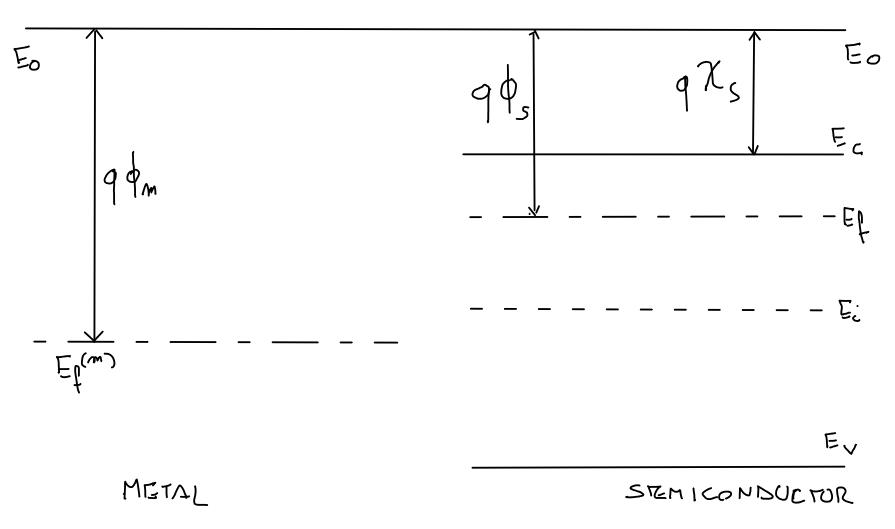
\includegraphics[width=0.5\textwidth]{ms1.png}
\end{wrapfigure}

Requirement for a Schottky diode are $E_f^{(m)}<E_f^{(s)}$ and a low doped semicondctor.\\
If we put the 2 materials toghether the distance between the difference $q\phi_m-q\chi_s=q\phi_{bn}$ is preserved in the semiconductor the bands goes up to align $E_f$ and we therefore have a built in potential $\phi_{bi}$. There is a diffusion process from semiconductor to metal and not in the opposite direction beacuse electrons of metal don't have enough energy.\\

\centering
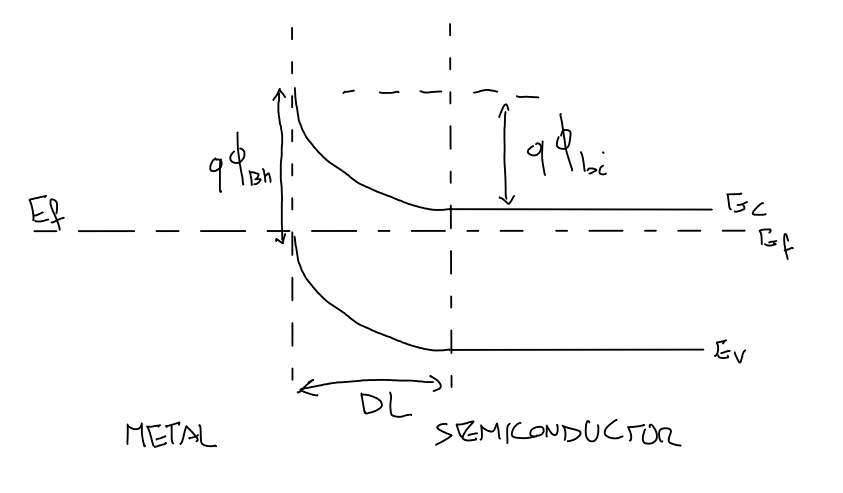
\includegraphics[width=0.5\textwidth]{ms2.png}\\
\raggedright
  
We can also draw a graph of the electric field where we can view the deplition layer and the built in potential as area.\\
This device is an ideal unilateral $p^+-n$ junction; we have the depliton layer only in the n side. We can recove the expression from the diode   
\begin{equation}
W_d=\sqrt{\frac{2\varepsilon_{si}}{q}\frac{1}{N_d}\phi_{bi}}=x
\end{equation}  

\centering
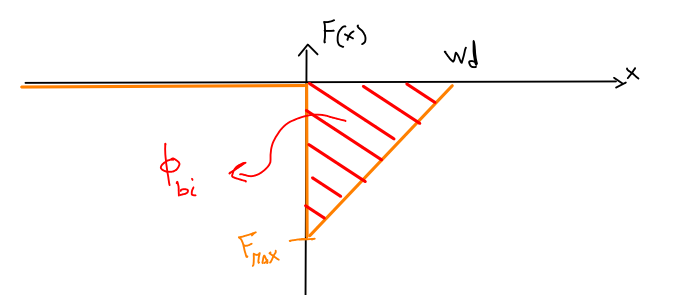
\includegraphics[width=0.5\textwidth]{ms3.png}\\
\raggedright

\subsection{Bias}
We will always consider the semiconductor part of the device n-doped and grounded; a voltage will be applied to the metal. As for the pn junction we consider foward bias if the voltage applied is grater than 0 and reverse bias if the voltage applied is less than zero.\\


\centering
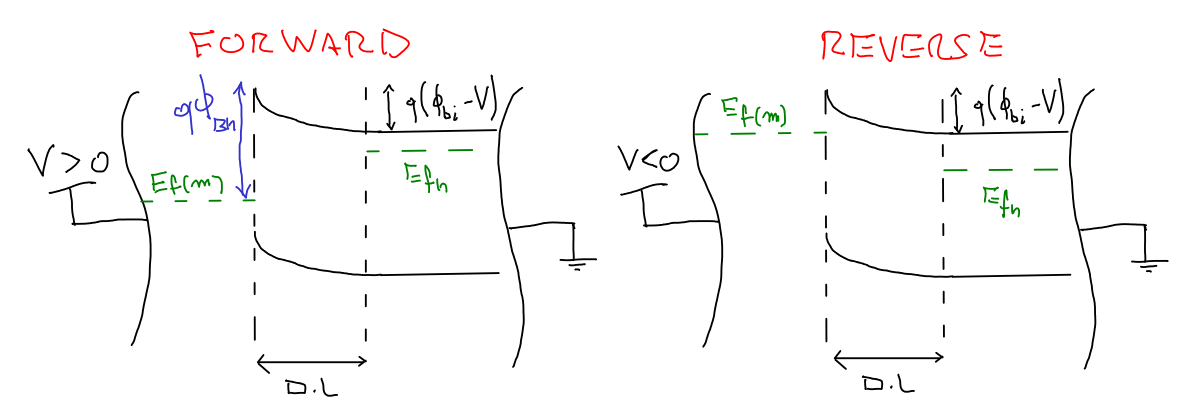
\includegraphics[width=0.55\textwidth]{msbias.png}\\
\raggedright


{\bf Reverse bias}\\
With reverse bias $E_{f(m)}$ becomes higher the depletion layer increases as the total voltage drop over the device.\\ 
{\bf Foward bias}\\
With foward bias $E_{f(m)}$ becomes lower, far from the contact we will have in the semiconductor a quasi-neutral region ,near the contact a transition zone with a depletion region. The total voltage drop decreases as the width of the depletion region.\\
We have two major difference with the pn junction: the flow of electrons from the semiconductor to the metal  don't have a minority constrain (the metal is full of electrons) so we will expect a high current but the transport of holes from metal to semiconductor has this limitation (the semiconductor is n-doped). $J_p$ will be small, negligible with respect to electrons flow.\\
Metal-semiconductor junction is a majority carrier device we won't deal with minority carrier in current transport phenomena. We will always neglect G-R processes beacuse are relevant only at low current regime.\\
%------------------------------------------------------------------------%
\subsection{Schottcky model}
%------------------------------------------------------------------------%
\centering
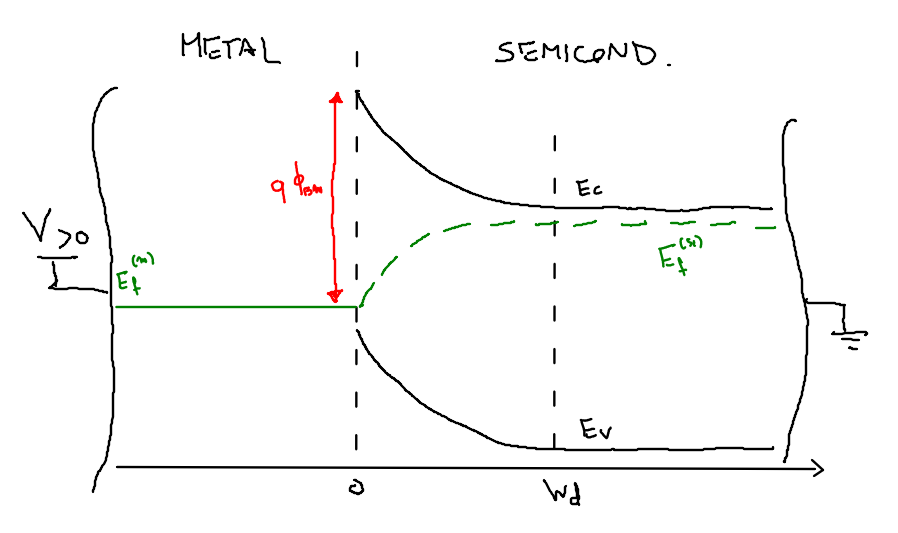
\includegraphics[width=0.45\textwidth]{shk.png}\\
\raggedright

We don't know the behaviour of $E_{fn}$ in the depletion layer but we know that in that zone we have the lower concetration of electrons so it can't be flat. Under stationary condition we can say that $ J_n=qn\mu_nF+qD_n \frac{dn}{dx}=$ constant and, as boundary condition, that $n(W_d)=N_d$ $n(0)=N_ce^{\frac{q\phi_{bn}}{kT}}$. F is given $-\frac{qN_d}{\varepsilon_{si}}(W_d-x)$ the only parameter we don't know is n and $\frac{dn}{dx}$ so solving the continuity equation for electrons with this boundary conditions we can get that
\begin{equation}
J=J_0(e^{\frac{qV}{kT}}-1)
\end{equation}
that is a relation identical to the pn junction but with a different $J_0$.\\
However this relation does not mach the experimental results. This is due to an implicit assumption that we've made using $n(0)=N_ce^{\frac{q\phi_{bn}}{kT}}$ as boundary condition; this happens only if the interface is always at thermodynamic equilibrium.\\
This model is valid for low mobility semicondutors (not for Si, Ge and GaAs).\\
%------------------------------------------------------------------------%
\subsection{Bethe's model}
%------------------------------------------------------------------------%
\begin{wrapfigure}{i}{0pt}
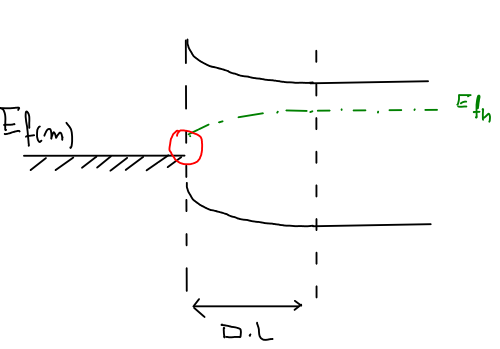
\includegraphics[width=0.25\textwidth]{msne.png}
\end{wrapfigure}

$E_{fn}$ can arrive at the interface higher than $E_{f(m)}$. We have a very thin interface that is of the order of fractions of nm there we can't describe current transport with drift and diffusion theory beacuse they're dominated by scattering events that occurs in tens of nanometers. We have to use a thermoionc transport model.\\
The electrons that pass from semiconductor to metal are that with an energy greater than $q(\phi_{bi}-V)$ so an energy higher than the potential barier of the depletion layer.\\
From energy dispersion relation $E=E_c+\frac{\hslash^2k^2}{2m_x}+\frac{\hslash^2k^2}{2m_y}+\frac{\hslash^2k^2}{2m_z}$ we define $E_x=\frac{\hslash^2k^2}{2m_x}$ the energy related to x transport and let's take into account only one ellipsoide.\\

\begin{wrapfigure}{i}{0pt}
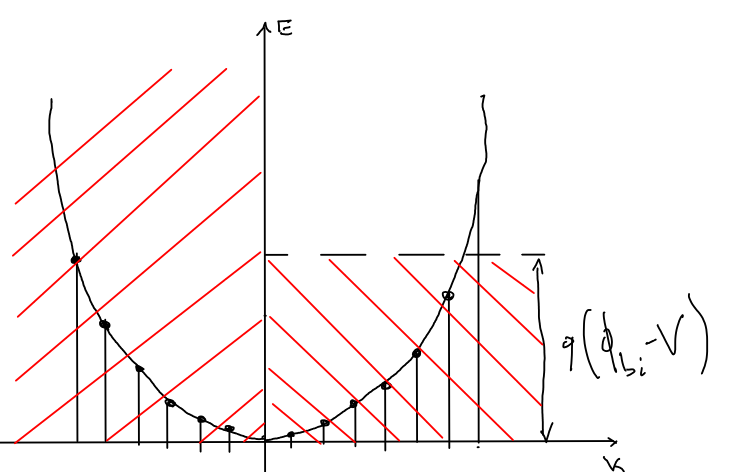
\includegraphics[width=0.25\textwidth]{bethe.png}
\end{wrapfigure}

Refering to the interface between the depletion layer and the quasi neutral region, half of the $E_x$ parabola can be neglected beacuse we want electrons that move from right to left (semiconductor to metal). We want also to consider only electrons with energy higher than $q(\phi_{bi}-V)$ so with a $k_x>\overline{k}$ so we can neglect other states.\\
The equivalent current of this electrons will be 
\begin{equation}
J_{s-m}^{(1)}=\sum_{k_x>\overline{k}}2 \frac{q}{L^3}v_x(k_x)f(k_x,k_y,k_z)
\end{equation}
the 2 factor is a spin correction. Adding a corrective term we can transform the summation into an integral 
\begin{equation}
J_{s-m}^{(1)}=\frac{1}{(\frac{2\pi}{L})^3}\int_{\overline{k_x}}^{+\infty}\int_{-\infty}^{+\infty}\int_{-\infty}^{+\infty}\frac{q}{L^3}v_x(k_x)f(k_x,k_y,k_z)dk_xdk_ydk_z
\end{equation}
remembering that $\hslash k_{x,y,z}=m_{x,y,z}v_{x,y,z}$ therefore $dk_{x,y,z}=\frac{m_{x,y,z}}{\hslash}dv_{x,y,z}$, we can change integration variable as 
\begin{equation}
J_{s-m}^{(1)}=\frac{2q}{(2\pi)^3}\int^{+\infty}_{v_x}\int_{-\infty}^{+\infty}\int_{-\infty}^{+\infty}v_xf(k_x,k_y,k_z) \frac{m_xm_ym_z}{\hslash^3} dv_xdv_ydv_z
\end{equation}
for f we can use M-B approximation $f\simeq e^{-\frac{E-E_f}{kT}}$ using energy dispersion relation 
\begin{equation}
E=E_c+\frac{1}{2}m_xv_x^2+\frac{1}{2}m_yv_y^2+\frac{1}{2}m_zv_z^2
\end{equation}
the M-B equation becomes
\begin{equation}
f\simeq e^{-\frac{E_c-E_{fn}}{kT}}\cdot e^{-1/2\frac{m_xv_x^2}{kT}}\cdot e^{-1/2\frac{m_yv_y^2}{kT}}\cdot e^{-1/2\frac{m_zv_z^2}{kT}}
\end{equation}
so solving the 3 integral (the first is a gaussian $=\frac{kT}{m_x}e^{-\frac{m_xv_x^2}{kT}}$ second and third $=\sqrt{\frac{2kT\pi}{m_{y,z}}}$) we get 
\begin{equation}
J_{s-m}^{(1)}=\frac{4\pi q}{h^3}\sqrt{m_xm_y}(kT)^2e^{\frac{-\phi_{bn}}{kT}}e^{\frac{qV}{kT}}=A\cdot\sqrt{m_xm_y}T^2e^{\frac{-\phi_{bn}}{kT}}e^{\frac{qV}{kT}}
\end{equation}
where $A=\frac{4\pi qk^2}{h^3}=120 \frac{A^2}{cm^2 K^2}$ it's called the Richardson constant.\\

\begin{wrapfigure}{i}{0pt}
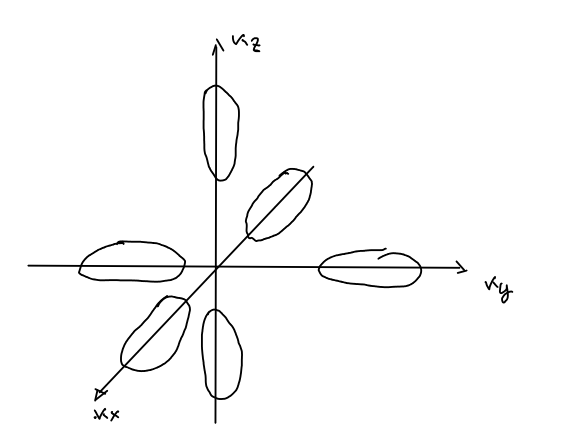
\includegraphics[width=0.2\textwidth]{ellips.png}
\end{wrapfigure}

Taking into account all the ellipsoide we get
\begin{equation}
J_{s-m}=A \frac{2m_t+4\sqrt{m_tm_l}}{m_0}T^2e^{\frac{-\phi_{bn}}{kT}}e^{\frac{qV}{kT}}=A^*T^2e^{\frac{-\phi_{bn}}{kT}}e^{\frac{qV}{kT}}
\end{equation}
with $A^*=A\cdot2.05$.\\
From m-s we can say that under th.eq the 2 current must be equal and that the barrier is costant equal to $q\phi_{bn}$ so $J_{m-s}=A^*T^2e^{\frac{-\phi_{bn}}{kT}}$.\\
So finally the total current throught the device will be 
\begin{equation}
J=A^*T^2e^{\frac{-q\phi_{bn}}{kT}}(e^{\frac{qV}{kT}}-1)=J_{0,th}(e^{\frac{qV}{kT}}-1)
\end{equation}
$\phi_{bn}$ it's a crucial parameter for current flow in metal semiconductor junction. We have a $J_{0,th}\simeq10^5 A/cm^2$ orders of magnitude higher with respect to the pn junction, a turn on voltage of 0.3-0.4 V and also a greater reverse bias current due to higher $J_0$.\\
This model is valid for high mobility semiconductors.\\
%------------------------------------------------------------------------%
\subsection{Universal model}
%------------------------------------------------------------------------%
We can connect the two models in an universal one.\\
Starting from Schottcky model we can use his assumption of $ J_n=qn\mu_nF+qD_n \frac{dn}{dx}=const$ and $n(W_d)=N_d$ but we have to change n(0). We can say something about $J_n(0)$ as the current density without scattering.

\begin{wrapfigure}{i}{0pt}
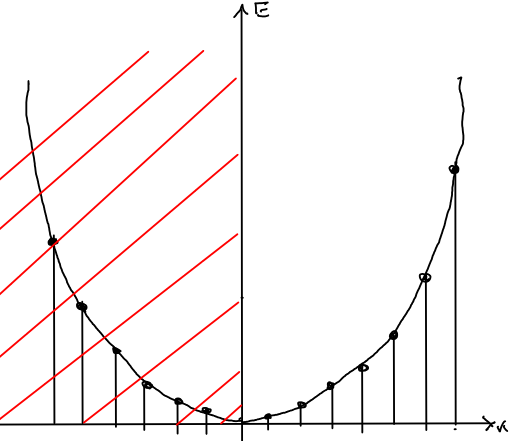
\includegraphics[width=0.2\textwidth]{generalmsmodel.png}
\end{wrapfigure}
 
We can calculate that term using energy dispersion relation but beacuse we are at the interface we will take all the left state of the parabola (we don't have a barrier) so we get 
\begin{equation}
J_n(0)=A^*T^2e^{-\frac{E_c-E_{fn}(0)}{kT}} 
\end{equation}
that is the correct boundary condition. If we muliply and divide this expression by $N_c$ we obtain
\begin{equation}
J_n(0)=A^*T^2 \frac{n(0)}{N_c}
\end{equation}
this for the electron flow from semiconductor to the metal. For the opposite direction we use the th.eq. condition and we get
\begin{equation}
J_n(0)=A^*T^2 \frac{n_0}{N_c}
\end{equation}
with $n_0$ electron concentration at the interface under th.eq.\\
So the final boundary condition is
\begin{equation}
J_n(0)=\frac{A^*T^2 }{N_c}[n(0)-n_0]
\end{equation}
We are using a drift-diffusion approach with thermionic boundary condition.\\
Solving this system we get an expression valid for all semiconductors that can be simplified in the 2 models depending on what type of semiconductor we have.\\
If mobility is large than it's easy to move electrons but difficult to remove them form the interface that becomes the bottom neck of the system. With low mobility it's difficult to move electrons but easy to remove them form the interfece so they don't pile up there.\\
%------------------------------------------------------------------------%
\subsection{Schottky effect}
%------------------------------------------------------------------------%
\begin{wrapfigure}{i}{0pt}
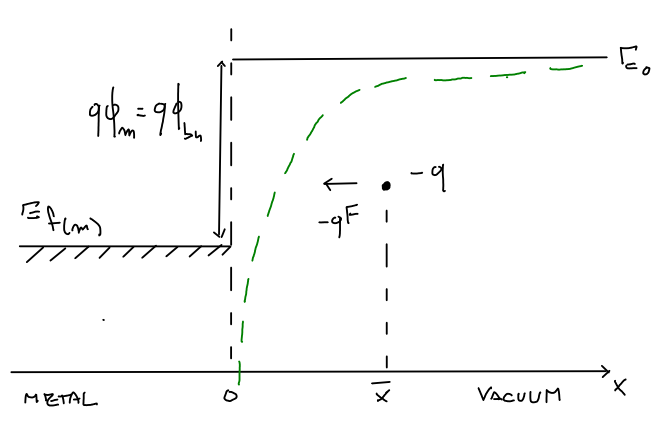
\includegraphics[width=0.4\textwidth]{scheff.png}
\end{wrapfigure}

The Schottky effect is a pure electrostatic effect that take place in the Bethe's model.\\
To study this effect we start from a metal-vacuum "junction" placing in the vacuum a single electron at a certain distance $\overline{x}$.\\
We have an electrostatic induction at the surface of the metal that attracts the electron in the vacuum near the surface. In order to calculate the electric field that attracts the single electron we can use the image method placing a positive charge +q at $-\overline{x}$ and removing the metal.\\
From this assumption we get 
\begin{equation}
-qF=\frac{1}{4\pi \varepsilon_0} \frac{-q^2}{(2\overline{x})^2}
\end{equation}
and so the electric field 
\begin{equation}
F=\frac{q}{16\pi\varepsilon_0x^2}
\end{equation}
from witch we can calculate ,integrating both part of the equation from x to $+\infty$, the potential as
\begin{equation}
\phi(x)=\phi(+\infty)+\frac{q}{16\pi \varepsilon_0 x}
\end{equation}
Multipling for -q we can obtain the energy 
\begin{equation}
E_0(x)=E_0(+\infty)-\frac{q^2}{16 \pi \varepsilon_0 x}
\end{equation}
and so the profile in green in the graph above.\\

\centering
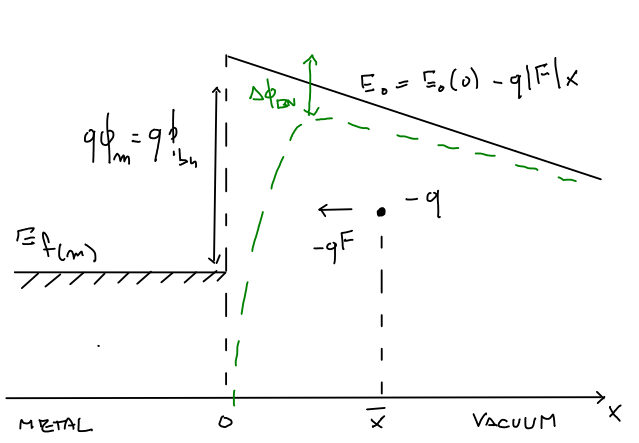
\includegraphics[width=0.35\textwidth]{deltaphibn.png}\\
\raggedright

If we consider that in the vacuum there is a costant electric field (and so $E_0(x)=E_0(0)-q|F|x$) like in figure beacuse the sistem is linear we obtain that
\begin{equation}
E_0(x)=E_0(0)-q|F|x-\frac{q^2}{16 \pi \varepsilon_0 x}
\end{equation}
and the behaviour in green in figure. We have change of the peak and so of the barrier that block our electrons. The $\Delta$ of the barrier is called Schottky barrier lowering.\\
We can calculate the new peak deriving by dx the $E_0(x)$ function finding the $x_{max}$ obtaining the energy at that point 
\begin{equation}
E_0(x_{max})=E_0(0)-\sqrt{\frac{q^3|F|}{4\pi \varepsilon_0}}
\end{equation}
So the difference in the barrier is $\Delta\phi_{bn}=\sqrt{\frac{q^3|F|}{4\pi \varepsilon_0}}$.\\
Now let's apply this effect on our metal semiconductor junction: when an electron travels throught the depletion layer from the semiconductor to the metal we have a barrier lowering of $\Delta\phi_{bn}=\sqrt{\frac{q^3|F_{max}|}{4\pi \varepsilon_{Si}}}$ (we place $F_{max}$ beacuse the maximum effect we have is with the max F and the narrower distance).\\
In our device we have a change of the J-V characteristic 
\begin{equation}
J=A^*T^2e^{\frac{-q(\phi_{bn}-\Delta\phi_{bn})}{kT}}(e^{\frac{qV}{kT}}-1)
\end{equation}
that creates an increment of $J_0$ and 2 opposit behaviour for reverse and forward bias: with $V<0$ the current increases increasing $|V|$, with $V>0$ J decrease this due to the dependance of $\Delta\phi_{bn}\propto\sqrt{F_{max}}\propto V_{rv-bias}$.\\
%------------------------------------------------------------------------%
\section{Ohmic contact}
%------------------------------------------------------------------------%
\begin{wrapfigure}{i}{0pt}
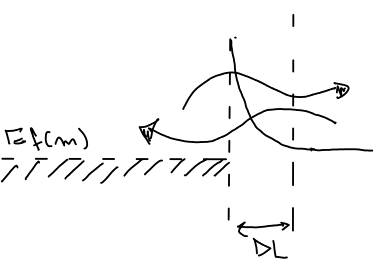
\includegraphics[width=0.15\textwidth]{tunnel.png}
\end{wrapfigure}

In order to have an ohmic contact we need a high doped semiconductor. With $N_d$ very high the depletion layer becomes narrower and increasing the doping concentration we arrive at a condition when there is a strong factor of J due to quantum-mechanical tunneling. That process does not depend on the type of bias so we don't have anymore a rectifing behaviour.\\

\centering
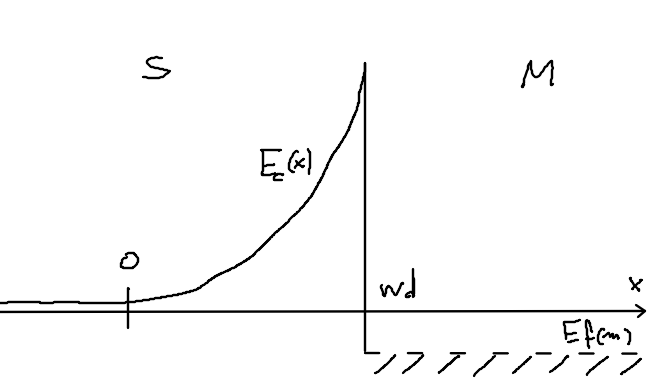
\includegraphics[width=0.35\textwidth]{1tunnel.png}\\
\raggedright

Taking into account the figure as reference system from the studied pn junction we know the behaviour of $E_c(x)=\frac{q^2N_d}{2\varepsilon_{Si}}x^2$ so we can calculate T ,transparancy coefficient as 
\begin{equation}
T=e^{-2\int_0^{W_d} Im\{E_c(x)\}dx}=e^{-2\int_0^{W_d} \sqrt{\frac{2m^*(E_c-E)}{\hslash^2}}dx}
\end{equation}
we have to remember that in this case $m^*$ is the effective mass for tunneling process. So if we consider $E=E_f$ (taken $E_f$ as reference the barrier is $E_c=\frac{q^2N_d}{2\varepsilon_{si}}x_n^2$)
\begin{equation}
T=e^{-2\int_0^{W_d} \sqrt{\frac{2m^*E_c}{\hslash^2}}dx}=e^{-2\sqrt{\frac{2m^*}{\hslash^2}}\sqrt{\frac{q^2N_d}{2\varepsilon_{Si}}}W_d^2/2}
\end{equation}
That substituiting $W_d$ with its expession we get
\begin{equation}
T=e^{-2\sqrt{\frac{2m^*}{\hslash^2}}\sqrt{\frac{q^2N_d}{2\varepsilon_{Si}}}\frac{2\varepsilon_{Si}}{qN_d}(\phi_{bi}-V)}=e^{-q \frac{(\phi_{bi}-V)}{E_{00}}}
\end{equation}
where $E_{00}=q\frac{\hslash \sqrt{N_d}}{2\sqrt{m^*\varepsilon_{si}}}$\\

\begin{wrapfigure}{i}{0pt}
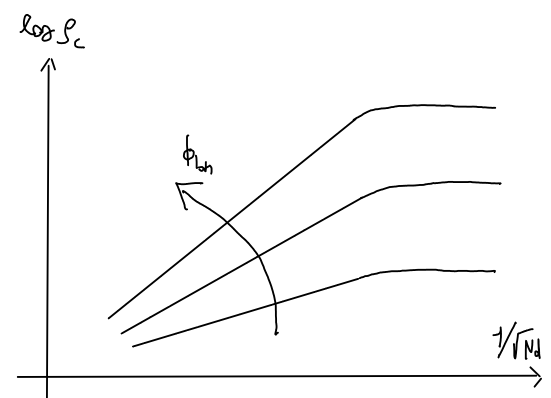
\includegraphics[width=0.3\textwidth]{contactrho.png}
\end{wrapfigure}

One important parameter of this device is the contact resistivity defined as 
\begin{equation}
\rho_c=(\frac{\partial J }{\partial V})^{-1}|_{V=0}=\frac{E_{00}}{q}e^{q\phi_{bi}/E_{00}}
\end{equation}
This parameter depends on the barrier hight and on $\sqrt{N_d}$. In the graph shows the $\log (\rho_c) - 1/\sqrt{N_d}$ dependance. It's a straight line until the concentration becomes too low and so tunneling effect is no more relevant.\\
To achive large current flow we need to perturbe only al little bit the device so it stays always near thermodynamic equilibrium.\\
The two figures below show how a contact is done in a device.

\centering
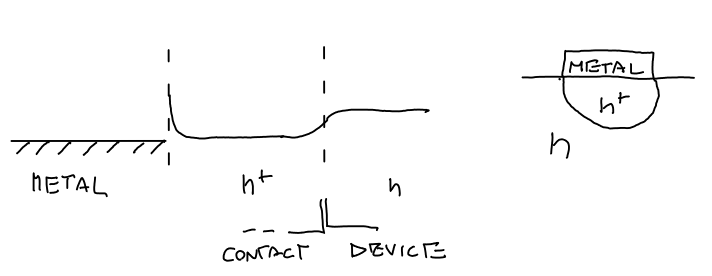
\includegraphics[width=0.5\textwidth]{ohmicconctact.png}\\
\raggedright

%------------------------------------------------------------------------%
\section{Interface states}
%------------------------------------------------------------------------%
We've always considered Si as a periodic infinite cristal but in metal-semiconductor junction we have the interface that interrupts the sequence of atoms. Some atoms of Si can't share all theyr 4 valence electrons creating some dangling bonds.\\

\begin{wrapfigure}{i}{0pt}
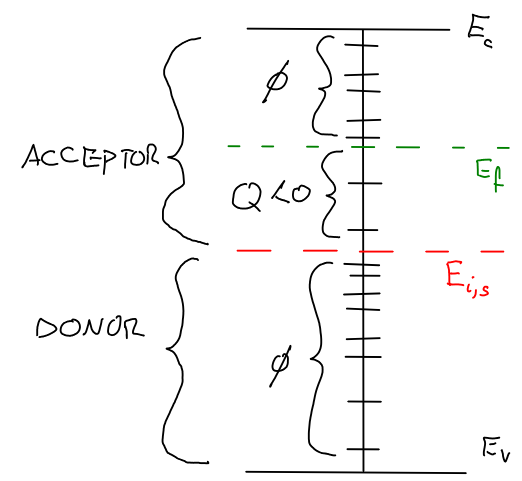
\includegraphics[width=0.3\textwidth]{is01.png}
\end{wrapfigure}

Electrons remains localize close to theyr silicon atoms this creates spurius energy level at the interface.\\ 
In the bulk region electrons and holes are only in the conduction band or in the valence band but at the interface can stay in a lot of states between this two bands.\\
The spurious states in the upper part of the bandgap have an acceptor behaviour (negativly charged when filled and neutral when empty) the others in the bottom part have a donor behaviour (neutral when filled and positivly charged when empty). The energy that divide this two type of states is the $E_{is}$.\\
All states below $E_f$ will be filled all the other states empty. So the previous band-diagram is incoherent with the Gauss'law since we have some exposed charge and no band banding.\\ 

\begin{wrapfigure}{i}{0pt}
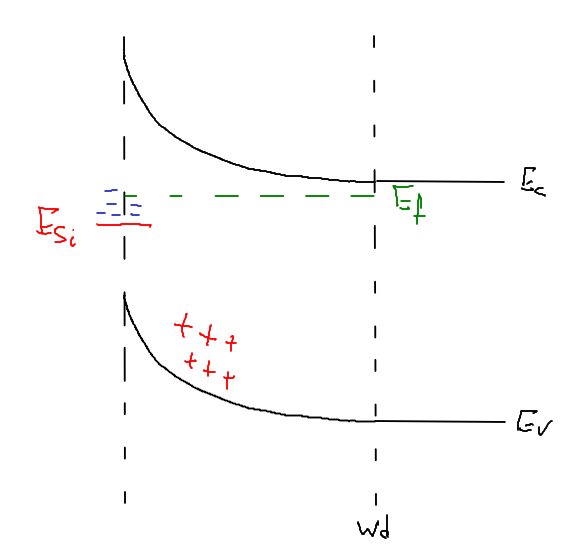
\includegraphics[width=0.19\textwidth]{is02.png}
\end{wrapfigure}

We have a negative charge so $\phi<0$ the bands band upward and the distance $E_f-E_{is}$ becomes narrower. The bands banding create a depletion region that expose a positive charge equal to the interface states' charge.\\
The distance between $E_c-E_f$ is not set only by doping concentration but also from interface states.\\
We define interface state density $N_{is} = [cm^{-2}eV^{-1}]$ in order to find the total charge introduced by the interface 
\begin{equation}
|Q_{is}|=N_{is}(E_f-E_{is})q
\end{equation}
The distance $E_c(0)-E_{is}\simeq E_{gap}/2$ so writing $\Delta E_{is}=E_c(0)-E_{is}\simeq E_{gap}/2$ we can say that
\begin{equation}
|Q_{is}|=N_{is}[\Delta E_{is}-(E_c(0)-E_{f})]q
\end{equation}
We know from the analysis of the pn junction that the charge in the depletion leyer is 
\begin{equation}
Q_{dep}=qN_dW_d=\sqrt{2\varepsilon_{si}qN_d\frac{E_c(0)-E_c(W_d)}{q}}
\end{equation}
where the last term is the voltage drop in the depletion layer.\\
For Gauss law this 2 terms have to be equal so solving the equation we get the level of the conduction band at the interface 
\begin{equation}
E_c(0)=\Delta E_{is}+\frac{\varepsilon_{si}N_d}{q^2N^2_{is}}-\sqrt{(\frac{\varepsilon_{si}N_d}{q^2N^2_{is}})^2+\frac{2\varepsilon_{si}N_d}{q^2N^2_{is}}(\Delta E_{is}-E_c(W_d))}
\end{equation}
This effect changes the barrerier hight and so theflow of current throught the device. $\phi_{bn}$ becomes strongly dependent on $N_{is}$

\subsection{Limit cases}
Starting from the equation $|Q_{is}|=Q_{dep}$ we have 2 limit cases.\\
$N_{is}=0$ in this case $E_c(0)=E_c(W_d)$ so we don't have a band banding we restore the ideal case.\\
$N_{is}\rightarrow +\infty$ in this case we notice that the first term has to be finite and so $\Delta E_{is}-(E_c(0)-E_{is}$ has to be zero that means that $E_c(0)=E_f+\Delta E_{is}$. \\
This case means we are moving $E_{f}$ up to $E_{is}$ that is totally indipendent from doping concentration but depends only from the interface states. This condition is called "Fermi level pinning at the surface".\\

The plot of $E_c(0)-\log(N_{is})$ make a transition between $10^{12}-10^{13}$ as order of magnitude.

\centering
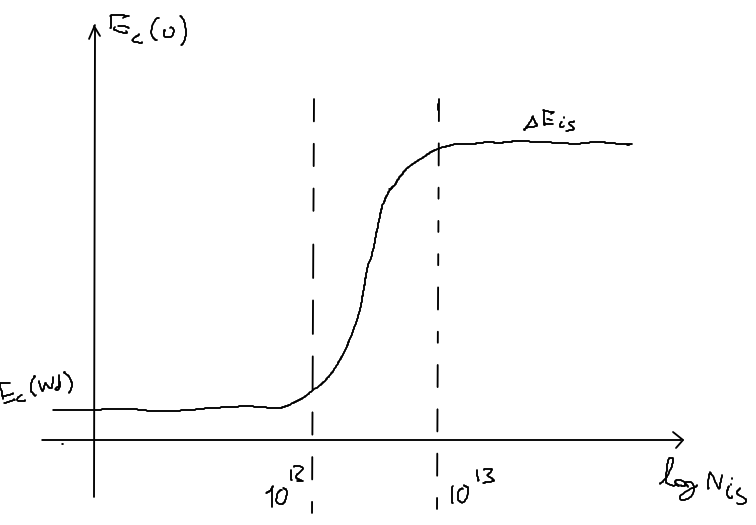
\includegraphics[width=0.35\textwidth]{is03.png}\\
\raggedright
















